\chapter{Hashfunktionen}\index{Hashfunktion}

Die Anforderungen an eine kryptographische Hashfunktion sind:
\begin{itemize}
    \item Kompression, d.h. ein beliebig langer Input wird auf einen Output fixer Länge gemappt
    \item Einwegfunktion (preimage resistance), d.h. gegeben $y = h(x)$ ist es schwierig, das verwendete $x$ zu bestimmen
    \item Schwache Kollisionsresistenz (2nd preimage resistance), d.h. gegeben $x$ mit $y = h(x)$ ist es schwierig, ein $x' \neq x$ zu finden, so dass $h(x) = h(x')$
    \item Starke Kollisionsresistenz (collision resistance), d.h. es ist schwierig, zwei $x$ und $x'$ zu finden, mit $x \neq x'$, so dass $h(x) = h(x')$
\end{itemize}

\section{Konstruktion}

Grundsätzlich sind für eine Hashfunktion zwei Komponenten nötig, eine Kompressionsfunktion, die längere Inputs auf die gewünschte Länge komprimieren, und ein Domain 
Extender, der aus Funktionen mit Eingaben fester Länge Funktionen mit Eingabe beliebiger Länge macht.

\paragraph{Kompressionsfunktionen}\index{Kompressionsfunktion}\index{Hashfunktion!Kompressionsfunktion} haben für einen fixen Input $m$ einen fixen Output $n$ mit 
$|m| > |n|$.

Es wird entweder eine eigens für den Hash geschriebene Funktion verwendet, z.B. bei MD5 und SHA-1, SHA-2, SHA-3, oder es wird ein Blockcipher eingesetzt. Bei einem 
Blockcipher wird ein Input der Länge $k+l$ (Länge des Schlüssels und Länge des Klartexts) auf einen Input der Länge $l$ gemappt. \\

Die zwei häufigsten Konstruktionen sind
\begin{itemize}
    \item Davis-Meyer: $h(x, y) = E_y(x) \oplus y$
    \item Miyaguchi-Preneel: $h(x, y) = E_x(y) \oplus x \oplus y$
\end{itemize}



\paragraph{Domain Extender}\index{Hashfunktion!Domain Extender}\index{Domain Extender} machen aus einer Funktion, die nur Inputs mit einer fixen Länge $n$ nimmt, eine 
Funktion die Inputs mit beliebiger Länge nimmt. 

Mehr oder weniger alle modernen Hashfunktionen folgen diesem Prinzip:

\begin{enumerate}
    \item Input wird in Blöcke $x_1, \ldots, x_n$ gleicher Länge aufgespalten
    \item Jeder Block dient als Input einer Einweg-Kompressionsfunktion $f$
    \item Input des $i$-ten Funktionsaufrufs sind das vorherige Ergebnis $h_{i-1}$ und der $i$-te Nachrichtenblock $x_i$
    \begin{itemize}
        \item $h_i = f(h_{i-1}, x_i)$
        \item $h(x) = h_{n+1}$ für eine Nachricht mit {n} Blöcken
        \item $h_i$ ist der interne Zustand der Hashfunktion
    \end{itemize}
    \item Ist die verwendete Funktion $f$ kollisionsresistent, so gilt das auch für $h$
    \item Im letzten Block der zu hashenden Nachricht wird die Länge der Originalnachricht angehängt, damit gleich endende aber unterschiedlich lange Nachrichten 
    unterschiedliche Hashwerte ergeben, z.B. \verb|Foo0| vs. \verb|Foo00|
    \item Grundproblem der Konstruktion: Length Extension Attack\index{Length Extension Attack}\index{Angriffe!Length Extension Attack}
    \begin{itemize}
        \item Kompletter interner State ist in Hashwert enthalten
        \item Falls MAC Konstruktion der Form H(key||Nachricht) ist, kann leicht Hashwert für verlängerte Nachricht konstruiert werden
    \end{itemize}
\end{enumerate}

\section{Algebraische Hashfunktionen}\index{Hashfunktion!algebraisch}

In der Praxis werden aus Geschwindigkeitsgründen hauptsächlich Hashfunktionen
basierend auf logischen Funktionen verwendet. Algebraische Funktionen sind kaum verbreitet, sie basieren auf ähnlichen Argumentationen wie
Public-Key Kryptographie (vgl. AES vs. RSA), also z.B. dem DLP (Discrete Logarithm Problem). Für die Hashfunktion gilt 

$$h(x) = g^x \mod p,$$

wobei das Umkehren der Funktion äquivalent zum Lösen des diskreten Logarithmusproblems ist.
Es gibt auch Hashfunktionen basierend auf RSA

$$H(x) = g^x \mod n (\text{mit } n = p\cdot q),$$

wo das Umkehren der Funktion äquivalent zum Lösen des RSA Problems ist.

\section{MD5}\index{MD5}\index{Hashfunktion!MD5} wurde 1991 von Ron Rivest als verbesserter Nachfolger zu MD4 erfunden.

\begin{itemize}
    \item 1996 erste Fehler entdeckt, 2004 weitere Schwachstellen gefunden
    \item 2007 Methoden vorgestellt, um 2 Dateien mit selber MD5 Checksumme zu erzeugen
    \item 2008 gefälschte SSL Zertifikate mit dieser Methode erzeugt
    \item 2008: ``Software developers, Certification Authorities, website owners, and users should avoid using the MD5 algorithm in any capacity. As previous research 
    has demonstrated, it should be considered cryptographically broken and unsuitable for further use.'' -- US-CERT, \url{http://www.kb.cert.org/vuls/id/836068}
\end{itemize}

Die Funktion erzeut in 64 Operationen (in 4 Runden zu je 16 Operationen) einen Output der Länge 128.

\begin{enumerate}
    \item Nachricht wird in 512 Bit große Blöcke aufgespalten und gepadded (siehe Kapitel ``Padding'')
    \item der interne State hat 128 Bit, wird in 4 32-Bit Wörtern gehalten. Er wird mit \verb|01 23 45 67|, \verb|89 ab cd ef|, \verb|fe dc ba 98|, \verb|76 54 32 10|, 
    sogenannte ``nothing up my sleeve'' numbers
    \item es gibt eine additive Rundenkonstante: in Runde $i$ wird $K_i = 2^{32}\cdot|\sin(i)|$ addiert 
    \item Alle 16 Operationen wechselt die Rundenfunktion ($F$, $G$, $H$, $I$)
    \begin{itemize}
        \item F(X,Y,Z) = (X and Y) or (not X and Z)
        \item G(X,Y,Z) = (X and Z) or (Y and not Z)
        \item H(X,Y,Z) = X $\oplus$ Y $\oplus$ Z
        \item I(X,Y,Z) = Y $\oplus$ (X or not Z)
    \end{itemize}
    \item Jede Runde um anderen Offset zirkulär geshiftet
\end{enumerate}

\begin{figure}[h]
    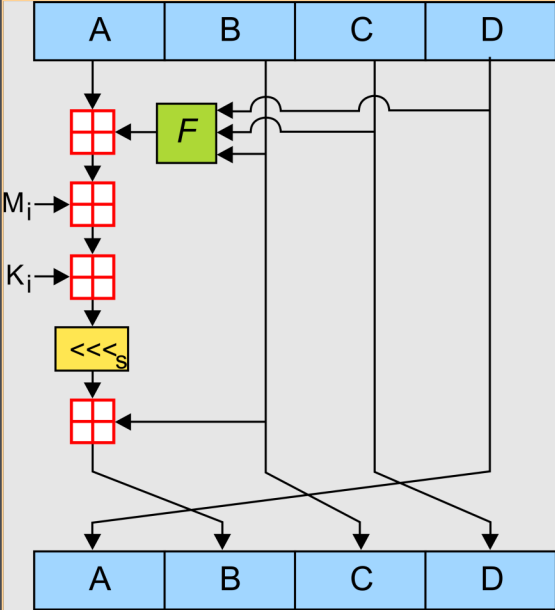
\includegraphics[width=0.4\textwidth]{figures/fig09-md5}
    \centering
    \caption{MD5 Operation, die 64 Mal wiederholt wird}
\end{figure}


\section{SHA (Secure Hash Algorithm)}\index{Hashfunktion!SHA}\index{SHA}

1993 wurde SHA-0 veröffentlicht, 1995 dann der verbesserte SHA-1 und 2001 SHA-2. Das NIST hat SHA-3 ausgeschrieben, das Ende des Auswahlprozesses war 2012 (vgl. AES).
Dann wurde Keccak als SHA-3 2015 standardisiert. \\

\paragraph{SHA-1}\index{SHA-1}
Der SHA-1 mit voller Rundenzahl gilt seit 2005 als unsicher. Kollisionen können mit $2^{63}$ Operationen erzeugt werden, 2008 wurde die Zahl auf $2^{51}$ verringert.
Seit 2017 sind Kollisionen in 2 validen PDF Dokumenten konstruierbar. \\

Er erzeugt einen 160 Bit Output und basiert auf denselben Grundideen wie MD4 und MD5:

\begin{itemize}
    \item Nachricht ebenfalls in 512-Bit Blöcke gespalten
    \item es gibt 80 Runden, alle 20 Runden wechselt die Rundenfunktion
    \begin{enumerate}
        \item F(X,Y,Z) = (X and Y) or (not X and Z) (ident zu MD5)
        \item G(X,Y,Z) = X $\oplus$ Y $\oplus$ Z (ident zu H aus MD5)
        \item H(X,Y,Z) = (X and Y) or (X and Z) or (Y and Z)
        \item I(X,Y,Z) = G (sic)
    \end{enumerate}
    \item es gibt 4 Rundenkonstanten
    \begin{enumerate}
        \item $K_1 = 230 \cdot \sqrt(2)$ 
        \item $K_2 = 230 \cdot \sqrt(3)$
        \item $K_3 = 230 \cdot \sqrt(5)$
        \item $K_4 = 230 \cdot \sqrt(10)$
    \end{enumerate}
    \item In jeder Runde um 30 zirkulär geshiftet
\end{itemize}

\paragraph{SHA-2}\index{SHA-2} beschreibt eine Familie an Hashfunktionen, die die Algorithmen SHA-224, SHA-256, SHA-384, SHA-512, SHA-512/224 und SHA-512/256. Sie sind im 
FIPS 
(Federal Information Processing Standards) PUB-180-4 beschrieben.


\begin{center}
    \begin{tabular}{ llll } 
        \hline
        Algorithmus & Ausgabegröße (Bit) & Interne Blockgröße (Bit) & basiert auf \\ 
        \hline
        SHA-224     & 224 &  512 & SHA-256\\
        SHA-256     & 256 &  512 & SHA-256\\
        SHA-384     & 384 & 1024 & SHA-512\\
        SHA-512     & 512 & 1024 & SHA-512\\
        SHA-512/224 & 224 & 1024 & SHA-512\\
        SHA-512/256 & 256 & 1024 & SHA-512\\
        \hline
    \end{tabular}
\end{center}

\subparagraph{SHA-224}: Kürzere Version von SHA-256 mit 224 Bit Ausgabelänge. Geeignet, wenn Speicher knapp ist, z.B. constraint devices (Memory).
\subparagraph{SHA-256}: Der meistverwendete SHA-2-Algorithmus. Standard für viele Anwendungen (z. B. TLS, digitale Signaturen)
\subparagraph{SHA-384}: Abgespeckte Version von SHA-512 mit anderer Initialisierung und kürzerer Ausgabe.
\subparagraph{SHA-512}: Sicherste (längste) Standardvariante mit 512 Bit Ausgabelänge.
\subparagraph{SHA-512/224} (constraint devices (Memory)), siehe SHA-512/256.  
\subparagraph{SHA-512/256} (allg. Sicherheit): Truncate-Versionen von SHA-512 mit kürzerer Ausgabelänge. Bietet eine Kombination aus höherer
Sicherheit (wegen 1024-Bit Blockgröße) und kürzeren Hashes.


\subparagraph{Merkle-Damgard}\index{Merkle-Damgard}\index{Hashfunktion!Merkle-Damgard}

Die Merkle-Damg\r{a}rd-Konstruktion (auch Merkles Meta-Verfahren) ist eine Methode zur Konstruktion von kryptographischen Hash-Funktionen, die auf Arbeiten von 
Ralph Merkle und Ivan Damg\r{a}rd zurückgeht.
Gegeben ist eine kollisionsresistente Kompressionsfunktion $f: \{0, 1\}^{a+b} \to \{0, 1\}^b$. Durch die Anwendung der Merkle-Damg\r{a}rd-Konstruktion ergibt sich daraus 
eine kollisionssichere Hash-Funktion $h: \{0, 1\}^* \to \{0, 1\}^b$, die beliebig lange Nachrichten auf einen Hashwert abbilden.

\begin{figure}[h]
    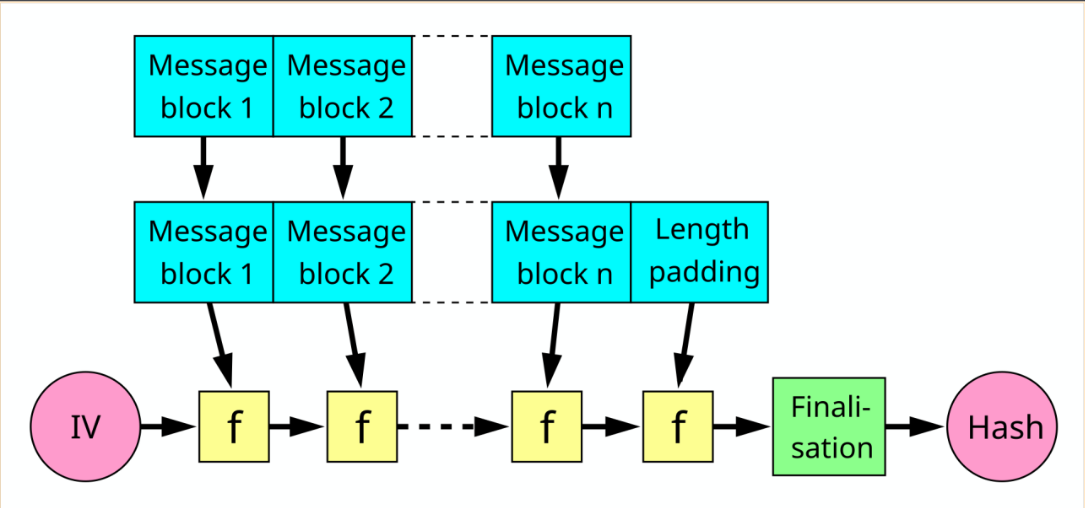
\includegraphics[width=0.9\textwidth]{figures/fig10-merkle-damgard}
    \centering
    \caption{Merkle-Damgard Hash}
\end{figure}

\begin{enumerate}
    \item Padding (Auffüllen): Die Eingabenachricht wird so erweitert, dass ihre Länge ein Vielfaches der Blockgröße ist. Dabei wird meist die ursprüngliche 
    Nachrichtenlänge am Ende angehängt.
    \item Aufteilung in Blöcke: Die aufgefüllte Nachricht wird in gleichgroße Blöcke unterteilt.
    \item Initialisierung: Ein fester Startwert (IV = Initialization Vector) wird gesetzt.
    \item Iterative Verarbeitung: Für jeden Block wird die Kompressionsfunktion angewendet:
    \begin{itemize}
        \item Eingabe: der aktuelle Block + der Ausgabewert des vorherigen Schritts
        \item Ausgabe: ein neuer Zwischenwert
    \end{itemize}
    \item Finales Ergebnis: Der Ausgabewert nach dem letzten Block ist der Hash-Wert.
\end{enumerate}

\subsection{SHA-3}\index{SHA-3}

2007 begann das NIST mit der Ausschreibung für einen Nachfolger von SHA-2. Am 2.10.2012 wurde Keccak (von Guido
Bertoni, Joan Daemen, Gilles Van Assche und Michaël Peeters) als Sieger verkündet und stellt die Basis für SHA-3 dar.

\begin{itemize}
    \item Verwendet im Unterschied zur bisherigen SHA Familie eine sog. ``Sponge''\index{Sponge}\index{SHA-3!Sponge} Konstruktion: ein 3-dimensionaler innerer Zustand 
    ($5\times 5\times w$-Bit Wörter; 
    bei $w =64$ sind das 1.600 Bits)
    \item Permutation: 24 Runden, 5 Schritte ($\theta, \rho, \pi, \chi, \iota$)
    \item Zuerst wird der zu hashende Text zur Gänze ``aufgesogen'' (absorbing phase)
    \item Danach der Hash gewünschter Länge ``ausgepresst'' (squeezing phase)
    \item Das ergibt Hashlängen von 224 bis 512 Bit (theoretisch aber beliebig lange, bis maximal 1.600); wird auch als Capacity Wert bezeichnet
\end{itemize}

\paragraph{Phasen}\index{Sponge!Phasen}

\begin{figure}[h]
    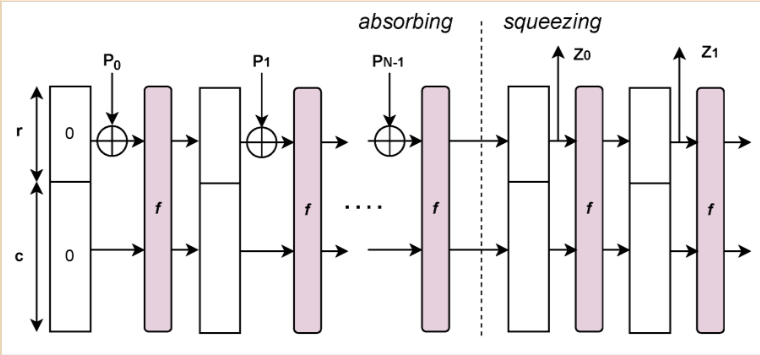
\includegraphics[width=0.75\textwidth]{figures/fig11-sponge}
    \centering
    \caption{SHA-3, Absorbing- und Squeezing Phase}
\end{figure}

\subparagraph{Absorbieren}\index{Sponge!Absorbieren}\index{Sponge!Absorbing Phase} Eingabedaten werden in Blöcke unterteilt.
Jeder Block wird mit dem internen Zustand (einer Art Speicher) verXORt.
Danach wird eine Permutation ($f$) auf den Zustand angewendet.

\subparagraph{Auspressen}\index{Sponge!Auspressen}\index{Sponge!Squeezing Phase} Nachdem alle Eingabeblöcke
absorbiert wurden, wird ein Teil des internen Zustands als Ausgabe extrahiert.
Bei langen Ausgaben (z.B. SHAKE-Funktionen) wird $f$ mehrfach ausgeführt, um mehr Output zu generieren.

\paragraph{State} Der interne Zustand in KECCAK hat die Breite $b=1600$ Bits (für SHA-3). Dieser Zustand ist aufgeteilt in ein 3D-Array mit
Dimensionen $5 \times 5 \times w$, wobei $w = 64$ bits. Jede Zelle $A[x][y]$ ist ein sogenanntes ``lane'' mit 64 Bits. 

\paragraph{Parameter}

Neben der Größe des States $b$, gibt es noch die Parameter

\begin{itemize}
    \item Rate $r$, wie viele Bits pro Sekunde verarbeitet werden können 
    \item Capacity $c$, wie groß die Sicherheitsreserve ist, sie berechnet sich als $c = b - r$. Bei Kapazität $c$  bietet der Algorithmus $c/2$ Bit Widerstand gegen 
    Kollisions- und Preimage-Attacken. \index{Collision Attack}\index{Preimage Attack}\index{Angriffe!Collision Attack}\index{!Preimage Attack}
\end{itemize}

Für den SHA-256 haben die Parameter $(b, r, c)$ dem Wert $(1600, 1088, 512)$.

\paragraph{Permutationsfunktion} KECCAK-f hat 24 Runden mit je 5 Steps:
\begin{enumerate}
    \item $\theta$ (theta) mischt jede Lane mit einer XOR-Mischung ihrer Spaltennachbarn.
    \item $\rho$ (rho) rotiert die Bits jeder Lane um einen bestimmten Wert.
    \item $\pi$ (pi) permutiert die Positionen der Lanes im $5\times 5$-Gitter.
    \item $\chi$ (chi) führt eine nichtlineare XOR-Maske aus, basierend auf anderen Werten in der Zeile.
    \item $\iota$ (iota) fügt einen Rundenkonstanten hinzu (zum Schutz vor symmetrischen Mustern).
\end{enumerate}

\noindent Diese Schritte garantieren Diffusion, Konfusion und Nichtlinearität, wie bei modernen
Blockchiffren.

\paragraph{Padding} Um sicherzustellen, dass die Nachricht gleichmäßig in $r$-Bit-Blöcke aufgeteilt werden
kann, ist ein Padding erforderlich. SHA-3 verwendet das Muster 100...001 (01 Padding), ein Bit mit Wert 1 wird gefolgt von null oder mehr 0-Bits (maximal $r-1$) und 
einem letzten 1-Bit.

\paragraph{XOFs}\index{XOF}\index{Extendable Output Function}\index{SHA-3!XOF} (Extendable Output Functions) basieren auf KECCAK und geben beliebig viele Ausgabebits 
zurück (nicht nur 256 oder 512).
Sie sind sehr flexibel für Anwendungen wie:
\begin{itemize}
    \item Key Derivation Function (KDF)
    \item Authentifizierung
    \item PQC Signaturen (z. B. SPHINCS+, Dilithium)
\end{itemize}

SHAKE bezeichnet den KECCAK Algorithmus, der er ein anderes Padding (1111 statt 01) und eine variable Ausgabelänge hat.


\section{Angriffe}\index{Hashfunktion!Angriffe}\index{Angriffe!Hashfunktion}

Sei $n$ die Länge des Outputs. Die Angriffe auf Hashfunktionen können wie folgt kategorisiert werden:

\begin{itemize}
    \item Angriff auf die Eigenschaft als Einwegfunktion: Idealerweise Komplexität von $O(2^n)$
    \item Angriff auf die schwache Kollisionsresistenz: Idealerweise Komplexität von $O(2^n)$ 
    \item Angriff auf die starke Kollisionsresistenz: Idealerweise Komplexität von $1.2\cdot 2^{n/2}$ (Geburtstagsparadoxon)
\end{itemize}

Generell gilt, ein Aufwand von $2^{80}$ ist ``schwierig''.

\paragraph{MD5} ist gebrochen.
\paragraph{SHA-1} ist gebrochen.
\paragraph{SHA-2} 

\begin{itemize}
    \item Output: 224/256/384/512 Bit
    \item Struktur: Merkle-Damgard
    \item Theoretische Angriffe auf rundenreduzierte Versionen bekannt
\end{itemize}

\paragraph{SHA-3}

\begin{itemize}
    \item Output: 224/256/384/512 Bit
    \item Struktur: Sponge
\end{itemize}

\subsection{BEAST Attack}\index{BEAST Attack}\index{Angriffe!BEAST}

Steht für \textbf{B}rowser \textbf{E}xploit \textbf{A}gainst \textbf{S}SL/\textbf{T}LS.
\begin{itemize}
    \item MitM Angriff und Chosen Plaintext Attack
    \item Record Splitting
    \item CBC Mode mit unsicherer IV-Generierung
    \item Beschrieben in CVE-2011-3389
    \item TLS1.0
\end{itemize}

Der BEAST-Angriff nutzt die Tatsache aus, dass bei TLS 1.0 der
Initialisierungsvektor (IV) für die nächste Nachricht vorhersehbar ist:
Er ist nämlich der letzte verschlüsselte Block der vorherigen Nachricht.

Dadurch kann ein Angreifer über sogenannte Chosen-Plaintext-Angriffe (d. h. gezielt eingefügte Daten) Rückschlüsse auf vertrauliche
Inhalte wie Cookies ziehen. \\

\noindent Damalige temporäre Workarounds
\begin{itemize}
    \item RC4
    \item 0-length Packets
    \item 1/n-1 Packet-Splitting: 
    \begin{itemize}
        \item Erster Record (1 Byte): Enthält nur ein harmloses Byte (z. B. ein Leerzeichen oder ein kontrolliertes Zeichen).
        \item Zweiter Record (n-1 Bytes): Enthält den Rest der eigentlichen Nachricht (z.B. HTTP-Headers, Cookies usw.).
    \end{itemize}
\end{itemize}
 

\begin{figure}[h]
    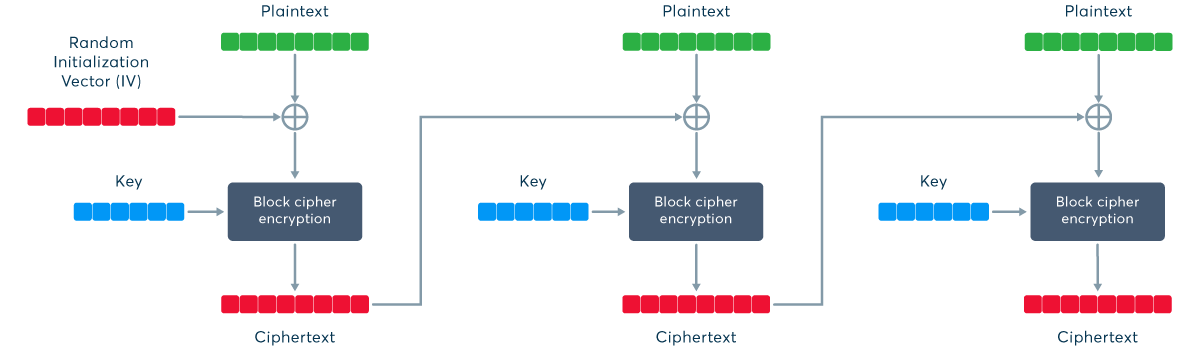
\includegraphics[width=0.9\textwidth]{figures/fig12-beast-attack-1}
    \centering
    \caption{How it should work: Proper encryption using a block cipher in CBC mode}
\end{figure}
\begin{figure}[h]
    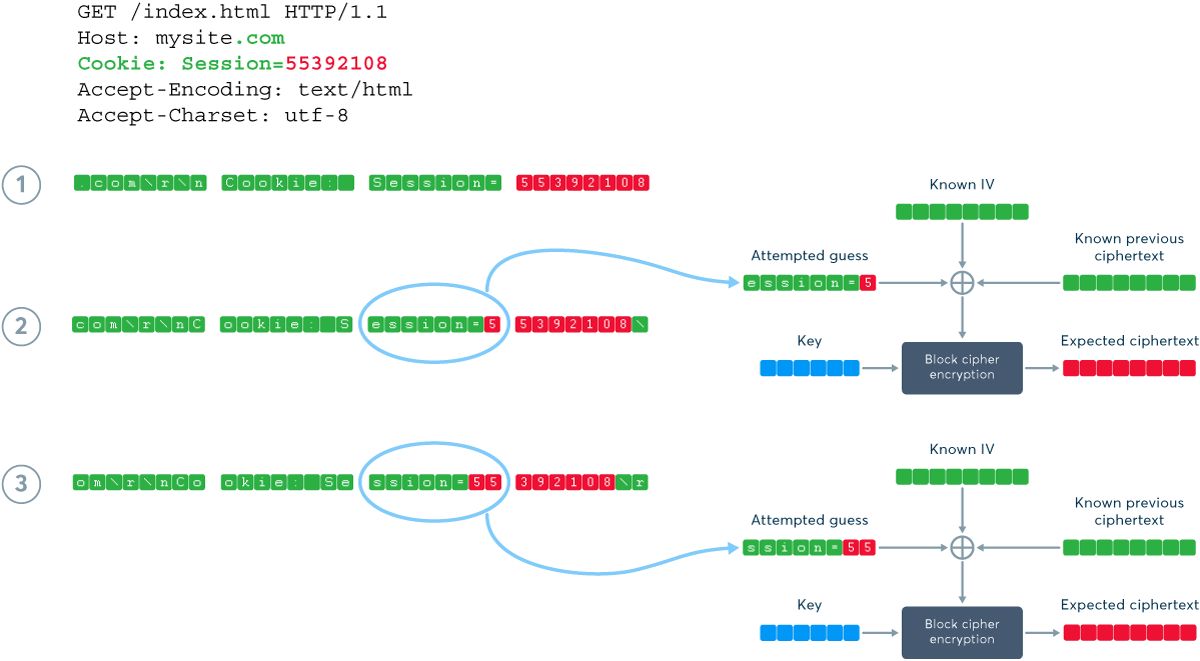
\includegraphics[width=0.9\textwidth]{figures/fig13-beast-attack-2}
    \centering
    \caption{The underlying vulnerability: A record splitting attack against TLS 1.0}
\end{figure}
\begin{figure}[h]
    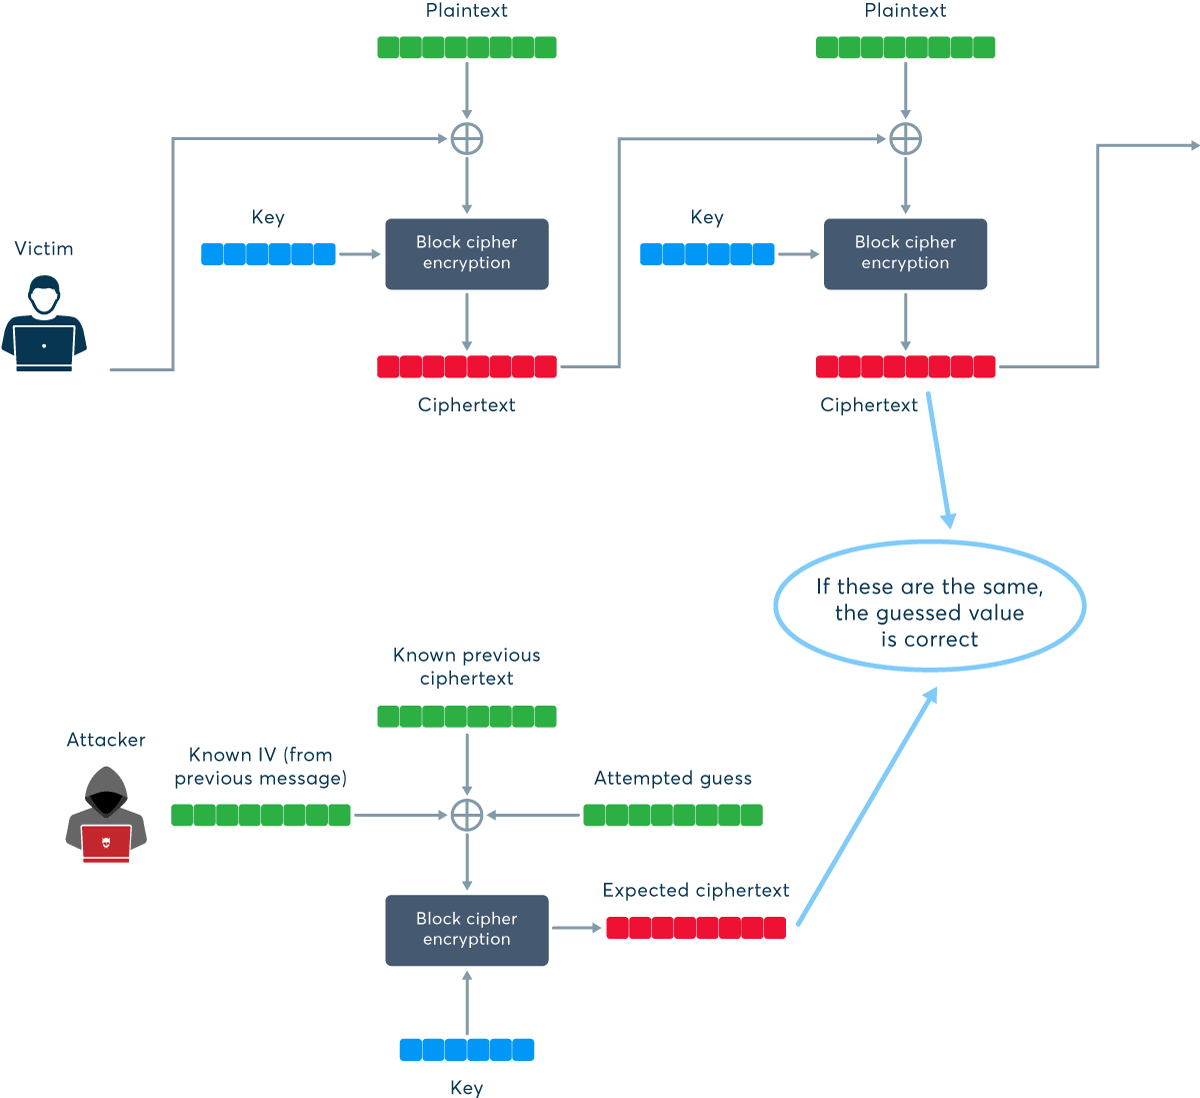
\includegraphics[width=0.9\textwidth]{figures/fig14-beast-attack-3}
    \centering
    \caption{The BEAST exploit: A chosen boundary attack combined with record splitting}
\end{figure}